\documentclass[11pt]{article}
\usepackage[margin = 1in]{geometry}
\usepackage{amsmath}
\usepackage{amssymb}
\usepackage{amsthm}
\usepackage{graphicx}
\usepackage{subfig}
\usepackage{enumitem}
\usepackage{url}
\usepackage[parfill]{parskip}
\usepackage{listings}
\newcommand{\cvector}[2]{\begin{pmatrix} #1 \\ #2 \end{pmatrix}}
\newcommand{\smatrix}[4]{\begin{pmatrix} #1 & #2 \\ #3 & #4 \end{pmatrix}}
\newcommand{\skipline}{\vspace{\baselineskip}}
\newenvironment{problem}[1]{\textbf{Problem #1: }}{\newpage}

% Options for packages loaded elsewhere
\PassOptionsToPackage{unicode}{hyperref}
\PassOptionsToPackage{hyphens}{url}
%
\usepackage{lmodern}
\usepackage{amssymb,amsmath}
\usepackage{ifxetex,ifluatex}
\ifnum 0\ifxetex 1\fi\ifluatex 1\fi=0 % if pdftex
\usepackage[T1]{fontenc}
\usepackage[utf8]{inputenc}
\usepackage{textcomp} % provide euro and other symbols
\else % if luatex or xetex
\usepackage{unicode-math}
\defaultfontfeatures{Scale=MatchLowercase}
\defaultfontfeatures[\rmfamily]{Ligatures=TeX,Scale=1}
\fi
% Use upquote if available, for straight quotes in verbatim environments
\IfFileExists{upquote.sty}{\usepackage{upquote}}{}
\IfFileExists{microtype.sty}{% use microtype if available
	\usepackage[]{microtype}
	\UseMicrotypeSet[protrusion]{basicmath} % disable protrusion for tt fonts
}{}
\makeatletter
\@ifundefined{KOMAClassName}{% if non-KOMA class
	\IfFileExists{parskip.sty}{%
		\usepackage{parskip}
	}{% else
		\setlength{\parindent}{0pt}
		\setlength{\parskip}{6pt plus 2pt minus 1pt}}
}{% if KOMA class
	\KOMAoptions{parskip=half}}
\makeatother
\usepackage{xcolor}
\IfFileExists{xurl.sty}{\usepackage{xurl}}{} % add URL line breaks if available
\IfFileExists{bookmark.sty}{\usepackage{bookmark}}{\usepackage{hyperref}}
\hypersetup{
	pdftitle={MidtermCode},
	hidelinks,
	pdfcreator={LaTeX via pandoc}}
\urlstyle{same} % disable monospaced font for URLs
\usepackage[margin=1in]{geometry}
\usepackage{color}
\usepackage{fancyvrb}
\newcommand{\VerbBar}{|}
\newcommand{\VERB}{\Verb[commandchars=\\\{\}]}
\DefineVerbatimEnvironment{Highlighting}{Verbatim}{commandchars=\\\{\}}
% Add ',fontsize=\small' for more characters per line
\usepackage{framed}
\definecolor{shadecolor}{RGB}{248,248,248}
\newenvironment{Shaded}{\begin{snugshade}}{\end{snugshade}}
\newcommand{\AlertTok}[1]{\textcolor[rgb]{0.94,0.16,0.16}{#1}}
\newcommand{\AnnotationTok}[1]{\textcolor[rgb]{0.56,0.35,0.01}{\textbf{\textit{#1}}}}
\newcommand{\AttributeTok}[1]{\textcolor[rgb]{0.77,0.63,0.00}{#1}}
\newcommand{\BaseNTok}[1]{\textcolor[rgb]{0.00,0.00,0.81}{#1}}
\newcommand{\BuiltInTok}[1]{#1}
\newcommand{\CharTok}[1]{\textcolor[rgb]{0.31,0.60,0.02}{#1}}
\newcommand{\CommentTok}[1]{\textcolor[rgb]{0.56,0.35,0.01}{\textit{#1}}}
\newcommand{\CommentVarTok}[1]{\textcolor[rgb]{0.56,0.35,0.01}{\textbf{\textit{#1}}}}
\newcommand{\ConstantTok}[1]{\textcolor[rgb]{0.00,0.00,0.00}{#1}}
\newcommand{\ControlFlowTok}[1]{\textcolor[rgb]{0.13,0.29,0.53}{\textbf{#1}}}
\newcommand{\DataTypeTok}[1]{\textcolor[rgb]{0.13,0.29,0.53}{#1}}
\newcommand{\DecValTok}[1]{\textcolor[rgb]{0.00,0.00,0.81}{#1}}
\newcommand{\DocumentationTok}[1]{\textcolor[rgb]{0.56,0.35,0.01}{\textbf{\textit{#1}}}}
\newcommand{\ErrorTok}[1]{\textcolor[rgb]{0.64,0.00,0.00}{\textbf{#1}}}
\newcommand{\ExtensionTok}[1]{#1}
\newcommand{\FloatTok}[1]{\textcolor[rgb]{0.00,0.00,0.81}{#1}}
\newcommand{\FunctionTok}[1]{\textcolor[rgb]{0.00,0.00,0.00}{#1}}
\newcommand{\ImportTok}[1]{#1}
\newcommand{\InformationTok}[1]{\textcolor[rgb]{0.56,0.35,0.01}{\textbf{\textit{#1}}}}
\newcommand{\KeywordTok}[1]{\textcolor[rgb]{0.13,0.29,0.53}{\textbf{#1}}}
\newcommand{\NormalTok}[1]{#1}
\newcommand{\OperatorTok}[1]{\textcolor[rgb]{0.81,0.36,0.00}{\textbf{#1}}}
\newcommand{\OtherTok}[1]{\textcolor[rgb]{0.56,0.35,0.01}{#1}}
\newcommand{\PreprocessorTok}[1]{\textcolor[rgb]{0.56,0.35,0.01}{\textit{#1}}}
\newcommand{\RegionMarkerTok}[1]{#1}
\newcommand{\SpecialCharTok}[1]{\textcolor[rgb]{0.00,0.00,0.00}{#1}}
\newcommand{\SpecialStringTok}[1]{\textcolor[rgb]{0.31,0.60,0.02}{#1}}
\newcommand{\StringTok}[1]{\textcolor[rgb]{0.31,0.60,0.02}{#1}}
\newcommand{\VariableTok}[1]{\textcolor[rgb]{0.00,0.00,0.00}{#1}}
\newcommand{\VerbatimStringTok}[1]{\textcolor[rgb]{0.31,0.60,0.02}{#1}}
\newcommand{\WarningTok}[1]{\textcolor[rgb]{0.56,0.35,0.01}{\textbf{\textit{#1}}}}
\usepackage{graphicx,grffile}
\makeatletter
\def\maxwidth{\ifdim\Gin@nat@width>\linewidth\linewidth\else\Gin@nat@width\fi}
\def\maxheight{\ifdim\Gin@nat@height>\textheight\textheight\else\Gin@nat@height\fi}
\makeatother
% Scale images if necessary, so that they will not overflow the page
% margins by default, and it is still possible to overwrite the defaults
% using explicit options in \includegraphics[width, height, ...]{}
\setkeys{Gin}{width=\maxwidth,height=\maxheight,keepaspectratio}
% Set default figure placement to htbp
\makeatletter
\def\fps@figure{htbp}
\makeatother
\setlength{\emergencystretch}{3em} % prevent overfull lines
\providecommand{\tightlist}{%
	\setlength{\itemsep}{0pt}\setlength{\parskip}{0pt}}
\setcounter{secnumdepth}{-\maxdimen} % remove section numbering


\begin{document}
	
	\begin{center}
		\textbf{Midterm} \\
		\textbf{Intro Math Modeling} \\
		\textbf{Math 336} \\
		\textbf{Stephen Giang RedID: 823184070} \\
		\skipline \skipline
	\end{center}

	\begin{problem}{1}
		\begin{figure}[h!]
			\centering
			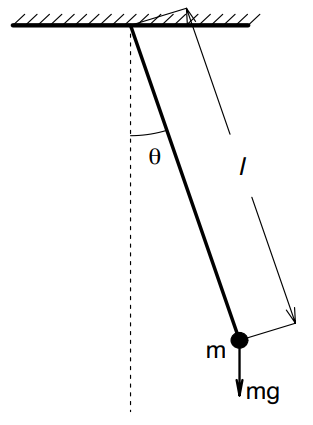
\includegraphics[height = 5cm]{Fig1.png}
			\caption{Simple pendulum of mass $m$ and length $l$ under the action of Earth’s gravitational force.}
		\end{figure}
		\begin{enumerate}[label = (\alph*)]
			\item Figure 1 shows a simple pendulum with mass $m$ , string length $l$ , and the Earth gravitational acceleration $g$. Use the dimensional analysis method to determine the period $\tau$ of the pendulum as a function of $m$, $l$, $g$, determined up to a constant $\alpha$, i.e., $\tau = \alpha m^a l^b g^c$
			\begin{align*}
				[\tau] &= \alpha [m]^a [l]^b [g]^c \\
				T &= M^a L^b (LT^{-2})^c \\
				M^0L^0T^1&= M^a L^{b+c} T^{-2c}
			\end{align*}
			Now we can see $a = 0$, $c = -1/2$ and $b = 1/2$ to get this equality.  Thus our solution is:
			\[\boldsymbol{\tau = \alpha l^{1/2} g^{-1/2} } = \alpha\sqrt{\frac{l}{g}}\]
			\newpage
			\item Use the conservation law of energy to find an approximate value of $\alpha$ in Part (a) under the condition
			of $\sin x \approx x$ when $x$ is close to be zero.
			\\ \\
			Notice we can find our angle $\theta$ using a simple harmonic sine function, $A\sin(\omega t + B )$. Let the pendulum reach a max height at $A$ and let the pendulum be released at $t = 0$.  This will make $B = 1 /2$ because $\sin \frac{\pi}{2} = 1$.  Thus we get the following:
			\[\theta = A\sin\left(\frac{2\pi}{\tau} t + \frac{\pi}{2}\right)\]
			We can calculate the tallest height when $\theta = A$.  Also notice we can use the fact that for very small $x$, $\sin x = x$, so we get:
			\[h = l - l\cos A = l(1 - \cos A) = 2l\sin^2\left(\frac{A}{2}\right) = 2l\left(\frac{A}{2}\right)^2 = \frac{lA^2}{2}\]
			We can calculate the velocity at the lowest point when $\cos\left(\frac{2\pi}{\tau} t + \frac{\pi}{2}\right) = 1$
			\[v = l\,\frac{d\theta}{dt} = \frac{2l\pi A}{\tau}\cos\left(\frac{2\pi}{\tau} t + \frac{\pi}{2}\right) = \frac{2l\pi A}{\tau}\]
			Now through the conservation of energy, we know that the potential energy at the highest point is equal to the kinetic energy at the lowest point.
			\begin{align*}
				E_p = mgh = mg\left[\frac{lA^2}{2}\right] &= \frac{m}{2}\left[\frac{2l\pi A}{\tau}\right]^2 = \frac{1}{2}mv^2 = E_p \\
				\frac{1}{2} mglA^2 &= \frac{1}{\tau^2}2ml^2\pi^2A^2 \\
				\tau^2 &= \frac{4l\pi^2}{g} \\
				\tau &= 2\pi \sqrt{\frac{l}{g}}
			\end{align*}
			This means we get that:
			\[\boldsymbol{\alpha = 2\pi}\]
			\item  If the string length is increased to $1.02l$ due to expansion in a higher temperature environment, and
			its corresponding period is denoted by $\tau_2$. Express $\tau_2$ in terms of $\tau$ found in Part (a) of this problem.
			\[\boldsymbol{\tau_2 = 2\pi \sqrt{\frac{1.02l}{g}} = \sqrt{1.02}\,2\pi \sqrt{\frac{l}{g}} = \sqrt{1.02}\,\tau} \]
			\item Given that $l = 75$ [cm] and $g = 9.8$ [m/s], calculate $\tau$ with unit in second. Write down your steps.
			You can use a calculator or R to do the calculation. You do not need to submit your R code for this
			problem even if you use R here.

			\[\boldsymbol{\tau = 2\pi \sqrt{\frac{(l = 0.75\,m)}{(g = 9.8\,m / s)}} = 1.73819\,s}\]
		\end{enumerate}
	\end{problem}

	\begin{problem}{2}
		The SVD result of a matrix A is below
\begin{lstlisting}[language = R]
svdA=svd(A)

svdA$d
[1] 2.0 1.0

svdA$u
    [,1] [,2]
[1,]   0    1
[2,]   1    0

svdA$v
    [,1] [,2]
[1,] 0.0    1
[2,] 0.4    0
[3,] 0.9    0
\end{lstlisting}
		\begin{enumerate}[label = (\alph*)]
			\item Write down three matrices $U, D, V$ in the SVD formula $A = UDV'$ where $V'$ denotes the transpose matrix of $V$.
			\[\boldsymbol{A = UDV' = \begin{bmatrix} 0 & 1 \\ 1 & 0 \end{bmatrix} \begin{bmatrix} 2 & 0 \\ 0 & 1\end{bmatrix} \begin{bmatrix} 0 & 0.4 & 0.9 \\ 1 & 0 & 0	\end{bmatrix}}\]
			\item Use the SVD formula $A = UDV'$ to approximately recover the original matrix A by hand calculation for the multiplication of the three matrices. Show your work and steps. You can use a calculator to do your number multiplication, but you still need to show your work. You may use R to verify your solution, but that is not required.
			\\
			\begin{align*}
				A = UDV' &= \begin{bmatrix} 0 & 1 \\ 1 & 0 \end{bmatrix} \begin{bmatrix} 2 & 0 \\ 0 & 1\end{bmatrix} \begin{bmatrix} 0 & 0.4 & 0.9 \\ 1 & 0 & 0	\end{bmatrix} \\
				&= \begin{bmatrix} 0(2) + 1(0) & 0(0) + 1(1) \\ 1(2) + 0(0) & 1(0) + 0(1)\end{bmatrix}\begin{bmatrix} 0 & 0.4 & 0.9 \\ 1 & 0 & 0	\end{bmatrix} \\
				&= \begin{bmatrix} 0 & 1 \\ 2 & 0\end{bmatrix}\begin{bmatrix} 0 & 0.4 & 0.9 \\ 1 & 0 & 0	\end{bmatrix} \\
				&= \begin{bmatrix} 0(0) + 1(1) & 0(0.4) + 1(0) & 0(0.9) + 1(0) \\ 2(0) + 0(1) & 2(0.4) + 0(0) & 2(0.9) + 0(0) \end{bmatrix} \\
				&= \boldsymbol{\begin{bmatrix} 1 & 0 & 0 \\ 0 & .8 & 1.8\end{bmatrix} }
			\end{align*}
		\end{enumerate}
	\end{problem}

	\begin{problem}{3}
		\begin{enumerate}[label = (\alph*)]
			\item Derive a formula for the monthly mortgage payment $x$, expressed in terms of the
			principal amount $P$, monthly interest rate $r$, and total number of months of the loan $n$. Show your work
			and the detailed steps. The answer for this step is a formula.
			\begin{align*}
				P_1 &= P(1 + r) - x \\
				P_2 &= P(1 + r)^2 - x(1 + r) - x \\
				\vdots & \qquad \vdots \qquad \vdots \qquad \vdots \\
				P_k &= P(1 + r)^k - x(1 + r)^{k -1} - \cdots - x(1 + r) - x \\
				&= P(1 + r)^k - x\left(\frac{1 - (1 + r)^k}{1 - (1 + r)}\right)
			\end{align*}
			Because $n$ is the total number of months on the loan, then at $k = n$, $P_{k = n} = 0$. Thus we get the equation below:
			\[\boldsymbol{P_n = 0 = P(1 + r)^n - x\left(\frac{1 - (1 + r)^n}{1 - (1 + r)}\right) }\]
			\item Given the data: The principal amount (i.e., the total loan) is $P = \$250, 000$, the annual interest
			rate is 3.6\% (converted into the monthly rate 0.3\%), and the loan is to be paid off in 30 years (equivalent
			to 360 months). Use the above derived formula and the data to compute the monthly mortgage payment
			$x$ by a calculator or R. The answer should be an amount of money per month. You do not need to submit
			the R code for this problem.
			\begin{align*}
				P_{360} = 0 &= 250,000(1 + 0.003)^{360} - x\left(\frac{1 - (1 + 0.003)^{360}}{1 - (1 + 0.003)}\right) \\
				x &= 250,000(1 + 0.003)^{360} \times \frac{1 - (1 + 0.003)}{1 - (1 + 0.003)^{360}} \\
				&= \boldsymbol{\$1,136.61 / \textbf{month}}
			\end{align*}
			\item  If the annual rate is reduced to 2.9\% in the above data, what is the monthly mortgage payment?
			\\ \\
			Our monthly interest rate will be $r = 0.029 / 12$, so our monthly payment will be:
			\begin{align*}
				x &= 250,000(1 + (0.029 / 12))^{360} \times \frac{1 - (1 + (0.029 / 12))}{1 - (1 + (0.029 / 12))^{360}} \\
				&= \boldsymbol{\$1,040.57 / \textbf{month}}
			\end{align*}
			\item If the principal is increased to $P = \$270, 000$, the annual rate is 2.9\%, and the loan period is
			still 30 years, what is the monthly mortgage payment now?
			\begin{align*}
				x &= 270,000(1 + (0.029 / 12))^{360} \times \frac{1 - (1 + (0.029 / 12))}{1 - (1 + (0.029 / 12))^{360}} \\
				&= \boldsymbol{\$1,123.82 / \textbf{month}}
			\end{align*}
		\end{enumerate}
	\end{problem}

	\begin{problem}{4}
		\textbf{The R programming part}
		\begin{enumerate}[label = (\roman*)]
			\item Use R to solve the following linear equations for x, y, z:
			\[\begin{cases}
				-x + 2.9y  + z = & 1 \\
				-1.5x - y + z = & 2.1 \\
				2.2x + y - 4z = & 0
			\end{cases}\]
			Copy your R solution result to your R code as comment lines after \#. 
			\\ \\
			Notice we can solve this using a coefficient matrix, $A$, constant matrix, $b$, and our solution matrix, $X$:
			\[A = \begin{bmatrix}
				-1 & 2.9 & 1 \\ -1.5 & -1 & 1 \\ 2.2 & 1 & -4
			\end{bmatrix} \qquad b = \begin{bmatrix}
				1 \\ 2.1 \\ 0
			\end{bmatrix} \qquad X = \begin{bmatrix}
				x \\ y \\ z
			\end{bmatrix}\]
			Now we use R to solve $AX = b$ and get the following solutions:
			\\ 
\begin{Shaded}
\begin{Highlighting}[]
\CommentTok{# Problem 4i}

\NormalTok{A =}\StringTok{ }\KeywordTok{matrix}\NormalTok{( }\KeywordTok{c}\NormalTok{(}\OperatorTok{-}\DecValTok{1}\NormalTok{, }\FloatTok{-1.5}\NormalTok{, }\FloatTok{2.2}\NormalTok{, }\FloatTok{2.9}\NormalTok{, }\DecValTok{-1}\NormalTok{, }\DecValTok{1}\NormalTok{, }\DecValTok{1}\NormalTok{, }\DecValTok{1}\NormalTok{, }\DecValTok{-4}\NormalTok{), }\DataTypeTok{nrow =} \DecValTok{3}\NormalTok{)}
\NormalTok{b =}\StringTok{ }\KeywordTok{matrix}\NormalTok{( }\KeywordTok{c}\NormalTok{(}\DecValTok{1}\NormalTok{, }\FloatTok{2.1}\NormalTok{, }\DecValTok{0}\NormalTok{), }\DataTypeTok{ncol =} \DecValTok{1}\NormalTok{)}
\NormalTok{X =}\StringTok{ }\KeywordTok{solve}\NormalTok{(A,b)}
\KeywordTok{sprintf}\NormalTok{(}\StringTok{"x = \%.4f"}\NormalTok{, X[}\DecValTok{1}\NormalTok{]) }\CommentTok{# x = -2.2117}
\end{Highlighting}
\end{Shaded}

\begin{verbatim}
## [1] "x = -2.2117"
\end{verbatim}

\begin{Shaded}
\begin{Highlighting}[]
\KeywordTok{sprintf}\NormalTok{(}\StringTok{"y = \%.4f"}\NormalTok{, X[}\DecValTok{2}\NormalTok{]) }\CommentTok{# y = 0.0015}
\end{Highlighting}
\end{Shaded}

\begin{verbatim}
## [1] "y = 0.0015"
\end{verbatim}

\begin{Shaded}
\begin{Highlighting}[]
\KeywordTok{sprintf}\NormalTok{(}\StringTok{"z = \%.4f"}\NormalTok{, X[}\DecValTok{3}\NormalTok{]) }\CommentTok{# z = -1.2161}
\end{Highlighting}
\end{Shaded}

\begin{verbatim}
## [1] "z = -1.2161"
\end{verbatim}
		\newpage
		\item Figure 2 shows the history of the global average December mean temperature anomalies. Use R
		and the dataset {\fontfamily{qcr}\selectfont EarthTemperatureData.txt} or {\fontfamily{qcr}\selectfont EarthTemperatureData.csv} downloadable from BB’s Assignment/Midterm block (or from the instructor’s email) to plot a similar figure but
		for June and with the following requirements.
		\begin{enumerate}[label = (\alph*)]
			\item Replace “Samuel Shen” and “December” in the main title by your name and June.
			\item Change the curve’s color from black to purple and use {\fontfamily{qcr} \selectfont lwd=5}.
			\item Compute the linear trend of the June temperature anomalies for the entire time span from 1850
			to 2015.
			\item Change the linear trend line’s color from black to blue, and use {\fontfamily{qcr} \selectfont lwd=3} for the trend line.
			\item Change the text “December trend = 0.52 deg C/century” to “June trend = ?? deg /Century”, and
			use the trend calculated from Step c) in the position ”??”.
			\item Save your plot as a png file with the filename as “first2letters-of-your-last-name-temp.png”. If your
			{\fontfamily{qcr} \selectfont Compile Report ...} is successful, you do not need to do this figure saving step.
			\item Plot the histogram of the June temperature anomalies from 1850 to 2015. The title of the figure is
			“Histogram of the June Temperature Anomalies.” The x-label is “Temperature anomalies [deg C].” Save
			this figure as the above step (f) but with a file name “first2letters-of-your-last-name-histogram.png”
			\item Save all your work as a pdf file and combine all your work for this exam into a single pdf file
			\item  Submit both pdf and R files into BB.
		\end{enumerate}
		\newpage
\begin{Shaded}
\begin{Highlighting}[]
\CommentTok{# Problem 4ii}

\KeywordTok{setwd}\NormalTok{(}\StringTok{'C:/Users/Stephen Giang/Documents/Math336Files'}\NormalTok{)}
\NormalTok{readData =}\StringTok{ }\KeywordTok{read.csv}\NormalTok{(}\StringTok{'EarthTemperatureData.csv'}\NormalTok{)}

\NormalTok{xvals =}\StringTok{ }\KeywordTok{as.numeric}\NormalTok{(readData}\OperatorTok{$}\NormalTok{YEAR)}
\NormalTok{yvals =}\StringTok{ }\KeywordTok{as.numeric}\NormalTok{(readData}\OperatorTok{$}\NormalTok{JUN)}

\KeywordTok{plot}\NormalTok{(xvals, yvals, }\StringTok{'l'}\NormalTok{, }\DataTypeTok{col =} \StringTok{'purple'}\NormalTok{, }\DataTypeTok{lwd =} \DecValTok{5}\NormalTok{, }
     \DataTypeTok{xlab =} \StringTok{'Year'}\NormalTok{, }\DataTypeTok{ylab =} \StringTok{'Temperature [deg C]'}\NormalTok{, }
     \DataTypeTok{main =} \StringTok{'Stephen Giang}\CharTok{\textbackslash{}'}\StringTok{s plot of June temperature anomalies'}\NormalTok{)}

\NormalTok{linmod =}\StringTok{ }\KeywordTok{lm}\NormalTok{(yvals }\OperatorTok{~}\StringTok{ }\NormalTok{xvals)}
\KeywordTok{abline}\NormalTok{(linmod, }\DataTypeTok{col =} \StringTok{'blue'}\NormalTok{, }\DataTypeTok{lwd =} \DecValTok{3}\NormalTok{)}

\NormalTok{slope =}\StringTok{ }\NormalTok{linmod}\OperatorTok{\$}\NormalTok{coefficients[}\DecValTok{2}\NormalTok{] }\OperatorTok{*}\StringTok{ }\DecValTok{100} \CommentTok{# .4525051}
\KeywordTok{text}\NormalTok{(}\DecValTok{1900}\NormalTok{, }\FloatTok{0.4}\NormalTok{, }\StringTok{'June trend = 0.45 deg C/ century '}\NormalTok{)}
\end{Highlighting}
\end{Shaded}
		\begin{figure}[h!]
			\centering
			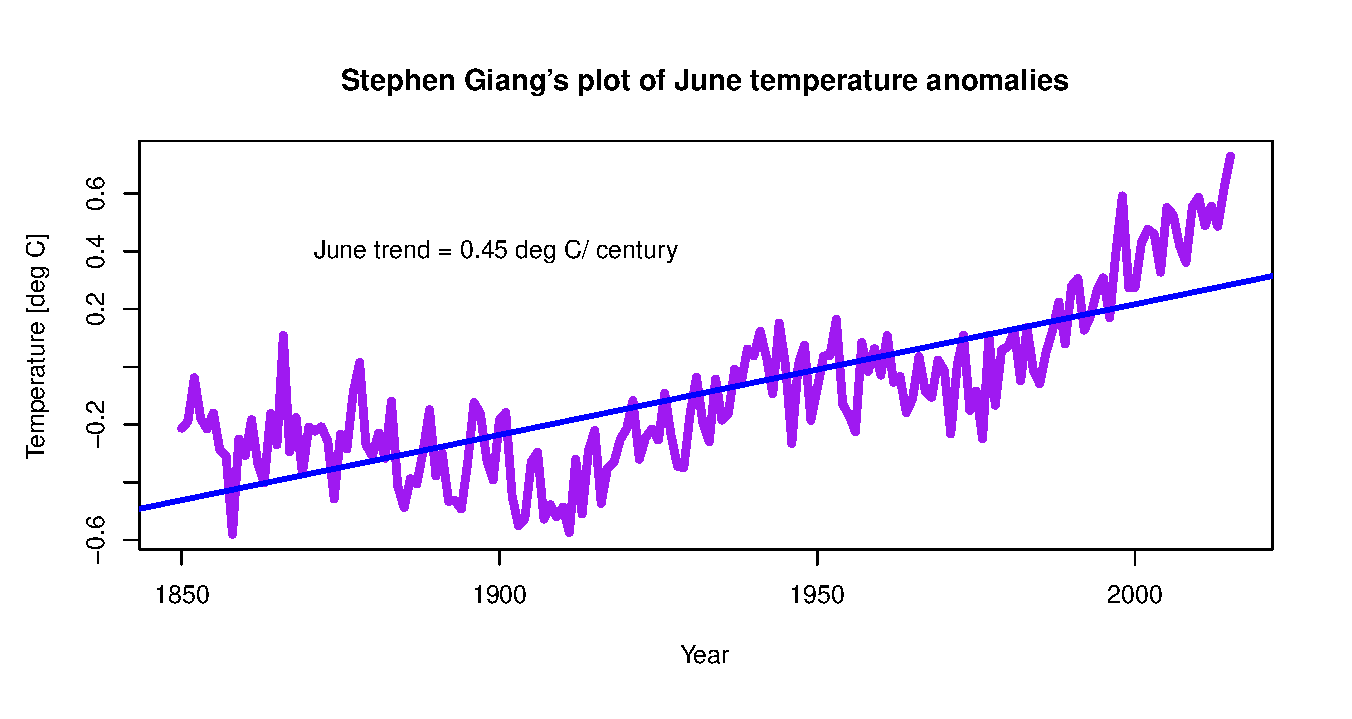
\includegraphics[height = 6cm]{SGTemp}
		\end{figure}
\begin{Shaded}
\begin{Highlighting}[]
\KeywordTok{hist}\NormalTok{(yvals, }\DataTypeTok{main =} \StringTok{'Histogram of the June Temperature Anomalies.'}\NormalTok{, }
     \DataTypeTok{xlab =} \StringTok{'Temperature anomalies [deg C]'}\NormalTok{)}
\end{Highlighting}
\end{Shaded}
		\begin{figure}[h!]
			\centering
			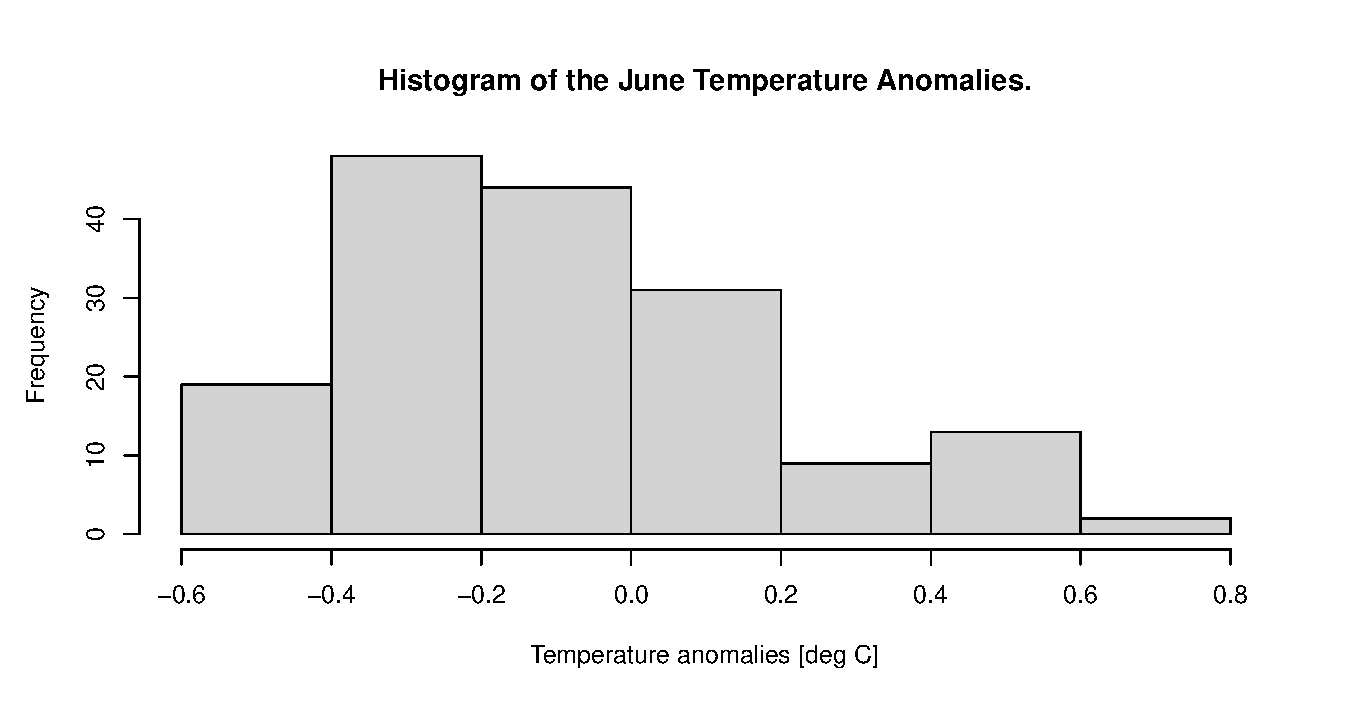
\includegraphics[height = 6cm]{SGHist}
		\end{figure}
		
		\end{enumerate}
	\end{problem}














\end{document}
